\subsection{Mesh > Scalar Field > Smooth}
\label{subsection:smoothMeshSF}

\begin{figure}[!htb]
\begin{center}
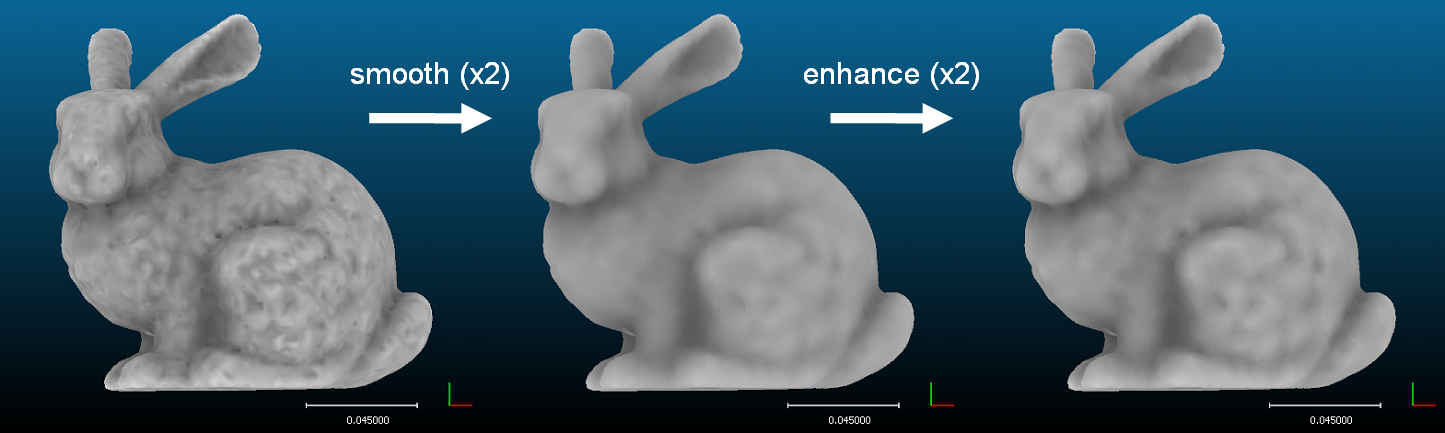
\includegraphics[width=0.9\textwidth]{Partie3_Fonctions/smoothAndEnhanceMeshSF.png}
\caption{\label{fig:smoothAndEnhanceMeshSF}Exemple de r�sultats obtenus avec les options \emph{smooth} et \emph{enhance} d'un champ scalaire port� par les sommets d'un maillage}
\end{center}
\end{figure}

\index{champ scalaire}
\index{lissage|see{filtrage}}
\index{filtrage}
Cette m�thode lisse spatialement les valeurs d'un champ scalaire port� par les sommets d'un maillage, en utilisant la topologie du maillage. La valeur scalaire au niveau d'un sommet est remplac�e par une moyenne (pond�r�e par la distance) des valeurs scalaires port�es par les sommets voisins.\\
\par
Remarque : cette fonction est beaucoup plus rapide que la fonction \emph{Gaussian filter}\index{filtrage!gaussien}
(section~\ref{subsection:scalarFieldGaussianFilter}) appliqu�e � un nuage de points non structur�. Elle ne permet par contre pas de r�gler la taille du \textit{noyau} de lissage.
